\emph{In problems 1--3, determine whether the given graph is connected or disconnected.}
\begin{center}
\begin{tabular}{c c c}
\parbox{1.5in}{\begin{enumerate}
\item \text{} \begin{center}
\begin{tikzpicture}[scale=0.7]
  \GraphInit[vstyle=simple]
  \tikzset{VertexStyle/.append style={scale=0.3}}
  \SetGraphUnit{2}
  
  \Vertex{a}
  \EA(a){b}
  \EA(b){c}
  \SO(a){d}
  \SO(b){e}
  
  \Edge(a)(d)
  \Edge(a)(e)
  \Edge(b)(c)
  \Edge(b)(d)
  \Edge(b)(e)
  \Edge(c)(e)
\end{tikzpicture}
\end{center}
\end{enumerate}}
&
\parbox{1.5in}{\begin{enumerate}
\setcounter{enumi}{1}
\item \text{} \begin{center}
\begin{tikzpicture}[scale=0.7]
  \GraphInit[vstyle=simple]
  \tikzset{VertexStyle/.append style={scale=0.3}}
  \SetGraphUnit{1}
  
  \Vertex{a}
  \NOEA(a){b}
  \EA(b){c}
  \EA(c){d}
  \EA(d){e}
  \EA(e){f}
  \EA(a){g}
  \EA(g){h}
  \EA(h){i}
  \EA(i){j}
  \EA(j){k}
  
  \Edge(a)(b)
  \Edge(b)(h)
  \Edge(h)(d)
  \Edge(d)(j)
  \Edge(j)(f)
  \Edge(g)(c)
  \Edge(c)(i)
  \Edge(i)(e)
  \Edge(e)(k)
\end{tikzpicture}
\end{center}
\end{enumerate}}
&
\parbox{1.5in}{\begin{enumerate}
\setcounter{enumi}{2}
\item \text{} \begin{center}
\begin{tikzpicture}[scale=0.7]
  \GraphInit[vstyle=simple]
  \tikzset{VertexStyle/.append style={scale=0.3}}
  \SetGraphUnit{2}
  
  \grEmptyCycle[RA=1.5,rotation=30,prefix=a]{6}
  
  \Edge(a0)(a2)
  \Edge(a2)(a4)
  \Edge(a4)(a0)
  \Edge(a1)(a3)
  \Edge(a3)(a5)
  \Edge(a5)(a1)
\end{tikzpicture}
\end{center}
\end{enumerate}}\\
\boxtext{Connected} & \boxtext{Disconnected} & \boxtext{Disconnected}
\end{tabular}
\end{center}

\emph{In problems 4--16, determine whether the given graph has an Euler circuit (and draw one if it exists).  If not, determine whether it has an Euler path (and draw one if so).}
\begin{enumerate}
\setcounter{enumi}{3}

\item \text{} \answer{Euler path: starting/ending at $a$/$d$} \begin{center} %4
\begin{tikzpicture}
  \GraphInit[vstyle=simple]
  \tikzset{VertexStyle/.append style={scale=0.3}}
  \SetGraphUnit{1.3}
  \Vertex{a}
  \SOEA(a){e}
  \NOEA(e){b}
  \SOWE(e){c}
  \SOEA(e){d}
  
  \extralabel{a}{90}{$a$}
  \extralabel{b}{90}{$b$}
  \extralabel{c}{-90}{$c$}
  \extralabel{d}{-90}{$d$}
  \extralabel{e}{-90}{$e$}
  
  \Edge(a)(b)
  \Edge(a)(e)
  \Edge(a)(c)
  \Edge(b)(d)
  \Edge(d)(c)
  \Edge(d)(e)
  \SetUpEdge[style={bend right=20}]
  \Edge(b)(e)
  \Edge(e)(b)
  \Edge(c)(e)
  \Edge(e)(c)
\end{tikzpicture}
\end{center}
\pagebreak

\item \text{} \answer{Euler path: starting/ending at $c$/$f$} \begin{center} %5
\begin{tikzpicture}
  \GraphInit[vstyle=simple]
  \tikzset{VertexStyle/.append style={scale=0.3}}
  \SetGraphUnit{0.9}
  \Vertex{a}
  \SOEA(a){b}
  \SOWE(b){d}
  \SOWE(a){f}
  \SOEA(d){c}
  \SOWE(d){e}
  
  \extralabel{a}{90}{$a$}
  \extralabel{b}{0}{$b$}
  \extralabel{c}{-90}{$c$}
  \extralabel{d}{135}{$d$}
  \extralabel{e}{-90}{$e$}
  \extralabel{f}{180}{$f$}
  
  \Edge(a)(b)
  \Edge(a)(d)
  \Edge(a)(f)
  \Edge(b)(c)
  \Edge(b)(d)
  \Edge(b)(f)
  \Edge(c)(d)
  \Edge(c)(e)
  \Edge(d)(e)
  \Edge(e)(f)
  \SetUpEdge[style={bend right=15}]
  \Edge(a)(e)
\end{tikzpicture}
\end{center}

\item \text{} \answer{Euler circuit} \begin{center} %6
\begin{tikzpicture}
  \GraphInit[vstyle=simple]
  \tikzset{VertexStyle/.append style={scale=0.3}}
  \SetGraphUnit{1.5}
  \Vertex{a}
  \EA(a){b}
  \EA(b){c}
  \SO(a){e}
  \SO(b){d}
  
  \extralabel{a}{90}{$a$}
  \extralabel{b}{90}{$b$}
  \extralabel{c}{0}{$c$}
  \extralabel{d}{-90}{$d$}
  \extralabel{e}{225}{$e$}
  
  \Edge(a)(b)
  \Edge(a)(e)
  \Edge(b)(c)
  \Edge(b)(d)
  \Edge(b)(e)
  \Edge(d)(e)
  \Edge(c)(e)
  \SetUpEdge[style={bend right=20}]
  \Edge(c)(d)
  \Edge(d)(c)
  \Edge(a)(e)
  \Edge(e)(a)
\end{tikzpicture}
\end{center}

\item \text{} \answer{Euler path: starting/ending at $b$/$c$} \begin{center} %7
\begin{tikzpicture}
  \GraphInit[vstyle=simple]
  \tikzset{VertexStyle/.append style={scale=0.3}}
  \SetGraphUnit{0.75}
  \Vertex{a}
  \NOEA(a){b}
  \SOEA(a){h}
  \SOEA(b){i}
  \NOEA(i){c}
  \SOEA(i){g}
  \SOEA(c){d}
  \EA(d){e}
  \SOEA(d){f}
  
  \extralabel{a}{180}{$a$}
  \extralabel{b}{90}{$b$}
  \extralabel{c}{90}{$c$}
  \extralabel{d}{45}{$d$}
  \extralabel{e}{0}{$e$}
  \extralabel{f}{-90}{$f$}
  \extralabel{g}{-90}{$g$}
  \extralabel{h}{-90}{$h$}
  \extralabel{i}{90}{$i$}
  
  \Edge(a)(b)
  \Edge(a)(h)
  \Edge(a)(i)
  \Edge(b)(c)
  \Edge(b)(i)
  \Edge(c)(d)
  \Edge(c)(i)
  \Edge(d)(e)
  \Edge(d)(f)
  \Edge(d)(g)
  \Edge(d)(i)
  \Edge(e)(f)
  \Edge(g)(i)
  \Edge(h)(i)
  \SetUpEdge[style={bend right=20}]
  \Edge(a)(d)
\end{tikzpicture}
\end{center}

\item \text{} \answer{No Euler circuit or path} \begin{center} %8
\begin{tikzpicture}
  \GraphInit[vstyle=simple]
  \tikzset{VertexStyle/.append style={scale=0.3}}
  \SetGraphUnit{1.3}
  \Vertex{a}
  \SOEA(a){b}
  \SO(b){c}
  \WE(c){d}
  \WE(d){e}
  \NO(e){f}
  
  \extralabel{a}{90}{$a$}
  \extralabel{b}{0}{$b$}
  \extralabel{c}{-90}{$c$}
  \extralabel{d}{-90}{$d$}
  \extralabel{e}{-90}{$e$}
  \extralabel{f}{180}{$f$}
  
  \Edge(a)(b)
  \Edge(a)(f)
  \Edge(b)(d)
  \Edge(b)(f)
  \Edge(c)(d)
  \Edge(d)(e)
  \Edge(e)(f)
\end{tikzpicture}
\end{center}

\item \text{} \answer{Euler circuit} \begin{center} %9
\begin{tikzpicture}
  \GraphInit[vstyle=simple]
  \tikzset{VertexStyle/.append style={scale=0.3}}
  \SetGraphUnit{1.2}
  \Vertex{a}
  \EA(a){b}
  \EA(b){c}
  \EA(c){d}
  \EA(d){e}
  \SO(a){f}
  \EA(f){g}
  \EA(g){h}
  \EA(h){i}
  \EA(i){j}
  \SO(f){k}
  \EA(k){l}
  \EA(l){m}
  \EA(m){n}
  \EA(n){o}
  
  \extralabel{a}{90}{$a$}
  \extralabel{b}{90}{$b$}
  \extralabel{c}{90}{$c$}
  \extralabel{d}{90}{$d$}
  \extralabel{e}{90}{$e$}
  \extralabel{f}{135}{$f$}
  \extralabel{g}{135}{$g$}
  \extralabel{h}{135}{$h$}
  \extralabel{i}{135}{$i$}
  \extralabel{j}{45}{$j$}
  \extralabel{k}{-90}{$k$}
  \extralabel{l}{-90}{$l$}
  \extralabel{m}{-90}{$m$}
  \extralabel{n}{-90}{$n$}
  \extralabel{o}{-90}{$o$}
  
  \Edge(a)(b)
  \Edge(a)(f)
  \Edge(b)(c)
  \Edge(b)(g)
  \Edge(c)(d)
  \Edge(c)(h)
  \Edge(c)(j)
  \Edge(d)(e)
  \Edge(d)(i)
  \Edge(e)(j)
  \Edge(f)(g)
  \Edge(f)(k)
  \Edge(f)(m)
  \Edge(g)(h)
  \Edge(g)(l)
  \Edge(h)(i)
  \Edge(h)(m)
  \Edge(i)(j)
  \Edge(i)(n)
  \Edge(j)(o)
  \Edge(k)(l)
  \Edge(l)(m)
  \Edge(m)(n)
  \Edge(n)(o)
  \SetUpEdge[style={bend right=40}]
  \Edge(d)(b)
  \Edge(l)(n)
\end{tikzpicture}
\end{center}

\item \text{} \answer{No Euler circuit or path} \begin{center} %10
\begin{tikzpicture}
  \GraphInit[vstyle=simple]
  \tikzset{VertexStyle/.append style={scale=0.3}}
  \grCycle[RA=1.5,prefix=a]{8}
  
  \extralabel{a0}{0}{$a$}
  \extralabel{a1}{45}{$b$}
  \extralabel{a2}{90}{$c$}
  \extralabel{a3}{135}{$d$}
  \extralabel{a4}{180}{$e$}
  \extralabel{a5}{225}{$f$}
  \extralabel{a6}{-90}{$g$}
  \extralabel{a7}{-45}{$h$}
  
  \Edge(a0)(a5)
  \Edge(a1)(a6)
  \Edge(a2)(a5)
  \Edge(a2)(a7)
  \Edge(a3)(a6)
  \Edge(a4)(a7)
\end{tikzpicture}
\end{center}

\item \text{} \answer{Euler circuit} \begin{center} %11
\begin{tikzpicture}
  \GraphInit[vstyle=simple]
  \tikzset{VertexStyle/.append style={scale=0.3}}
  \SetGraphUnit{1.3}
  \Vertex{a}
  \EA(a){b}
  \EA(b){c}
  \EA(c){d}
  \SO(d){e}
  \EA(e){f}
  \WE(e){g}
  \WE(g){h}
  \WE(h){i}
  
  \extralabel{a}{90}{$a$}
  \extralabel{b}{90}{$b$}
  \extralabel{c}{90}{$c$}
  \extralabel{d}{90}{$d$}
  \extralabel{e}{-90}{$e$}
  \extralabel{f}{-90}{$f$}
  \extralabel{g}{-90}{$g$}
  \extralabel{h}{-90}{$h$}
  \extralabel{i}{-90}{$i$}
  
  \Edge(a)(b)
  \Edge(a)(h)
  \Edge(a)(i)
  \Edge(b)(c)
  \Edge(b)(h)
  \Edge(b)(i)
  \Edge(c)(d)
  \Edge(c)(e)
  \Edge(c)(g)
  \Edge(c)(i)
  \Edge(d)(e)
  \Edge(d)(g)
  \Edge(d)(h)
  \Edge(e)(f)
  \Edge(g)(h)
  \Edge(h)(i)
  \SetUpEdge[style={bend right=30}]
  \Edge(c)(a)
  \Edge(h)(e)
  \Edge(f)(g)
\end{tikzpicture}
\end{center}

\item \text{} \answer{No Euler circuit or path} \begin{center} %12
\begin{tikzpicture}
  \GraphInit[vstyle=simple]
  \tikzset{VertexStyle/.append style={scale=0.3}}
  \SetGraphUnit{2.6}
  \Vertex{a}
  \EA(a){b}
  \SO(a){c}
  \SO(b){d}
  
  \extralabel{a}{90}{$a$}
  \extralabel{b}{90}{$b$}
  \extralabel{c}{-90}{$c$}
  \extralabel{d}{-90}{$d$}
  
  \tikzset{EdgeStyle/.style = {->-,>=latex[round]}}
  \Edge(a)(b)
  \Edge(a)(d)
  \Edge(c)(a)
  \Edge(c)(b)
  \Edge(d)(c)
  \tikzset{EdgeStyle/.style = {->-,>=latex[round],bend right=20}}
  \Edge(b)(d)
  \Edge(d)(b)
\end{tikzpicture}
\end{center}

\item \text{} \answer{Euler path: starting at $a$, ending at $e$} \begin{center} %13
\begin{tikzpicture}
  \GraphInit[vstyle=simple]
  \tikzset{VertexStyle/.append style={scale=0.3}}
  \SetGraphUnit{2}
  \Vertex{a}
  \EA(a){b}
  \EA(b){c}
  \SO(a){d}
  \EA(d){e}
  
  \extralabel{a}{90}{$a$}
  \extralabel{b}{90}{$b$}
  \extralabel{c}{0}{$c$}
  \extralabel{d}{-90}{$d$}
  \extralabel{e}{-90}{$e$}
  
  \tikzset{EdgeStyle/.style = {->-,>=latex[round]}}
  \Edge(a)(d)
  \Edge(a)(e)
  \Edge(b)(a)
  \Edge(d)(b)
  \tikzset{EdgeStyle/.style = {->-,>=latex[round],bend right=20}}
  \Edge(b)(c)
  \Edge(c)(b)
  \Edge(b)(e)
  \Edge(e)(b)
  \Edge(c)(e)
  \Edge(e)(c)
  \Edge(d)(e)
  \Edge(e)(d)
\end{tikzpicture}
\end{center}
\pagebreak

\item \text{} \answer{Euler path: starting at $c$, ending at $b$} \begin{center} %14
\begin{tikzpicture}
  \GraphInit[vstyle=simple]
  \tikzset{VertexStyle/.append style={scale=0.3}}
  \SetGraphUnit{2}
  \Vertex{a}
  \EA(a){b}
  \EA(b){c}
  \SO(a){d}
  \EA(d){e}
  \EA(e){f}
  
  \extralabel{a}{90}{$a$}
  \extralabel{b}{90}{$b$}
  \extralabel{c}{0}{$c$}
  \extralabel{d}{-90}{$d$}
  \extralabel{e}{-90}{$e$}
  \extralabel{f}{-90}{$f$}
  
  \tikzset{EdgeStyle/.style = {->-,>=latex[round]}}
  \Edge(a)(b)
  \Edge(b)(d)
  \Edge(b)(f)
  \Edge(c)(b)
  \Edge(c)(e)
  \Edge(e)(a)
  \Edge(e)(b)
  \Edge(f)(c)
  \Edge(f)(e)
  \tikzset{EdgeStyle/.style = {->-,>=latex[round],bend right=20}}
  \Edge(a)(d)
  \Edge(d)(a)
  \Edge(b)(c)
  \Edge(c)(b)
  \Edge(d)(e)
  \Edge(e)(d)
  \tikzset{EdgeStyle/.style = {->-,>=latex[round],bend right=30}}
  \Edge(d)(f)
\end{tikzpicture}
\end{center}

\item \text{} \answer{No Euler circuit or path} \begin{center} %15
\begin{tikzpicture}
  \GraphInit[vstyle=simple]
  \tikzset{VertexStyle/.append style={scale=0.3}}
  \SetGraphUnit{1.4}
  \Vertex{a}
  \EA(a){b}
  \EA(b){c}
  \EA(c){d}
  \SO(a){e}
  \EA(e){f}
  \EA(f){g}
  \EA(g){h}
  \SO(e){i}
  \EA(i){j}
  \EA(j){k}
  \EA(k){l}
  
  \extralabel{a}{90}{$a$}
  \extralabel{b}{90}{$b$}
  \extralabel{c}{90}{$c$}
  \extralabel{d}{90}{$d$}
  \extralabel{e}{135}{$e$}
  \extralabel{f}{135}{$f$}
  \extralabel{g}{135}{$g$}
  \extralabel{h}{45}{$h$}
  \extralabel{i}{-90}{$i$}
  \extralabel{j}{-90}{$j$}
  \extralabel{k}{-90}{$k$}
  \extralabel{l}{-90}{$l$}
  
  \tikzset{EdgeStyle/.style = {->-,>=latex[round]}}
  \Edge(a)(e)
  \Edge(b)(a)
  \Edge(b)(c)
  \Edge(c)(g)
  \Edge(d)(c)
  \Edge(e)(f)
  \Edge(f)(b)
  \Edge(f)(j)
  \Edge(g)(f)
  \Edge(g)(k)
  \Edge(h)(d)
  \Edge(h)(g)
  \Edge(i)(e)
  \Edge(j)(i)
  \Edge(j)(k)
  \Edge(k)(l)
  \Edge(l)(h)
\end{tikzpicture}
\end{center}

\item \text{} \answer{Euler path: starting at $d$ and ending at $b$} \begin{center} %16
\begin{tikzpicture}
  \GraphInit[vstyle=simple]
  \tikzset{VertexStyle/.append style={scale=0.3}}
  \SetGraphUnit{1.4}
  \Vertex{a}
  \SOEA(a){e}
  \NOEA(e){b}
  \SOEA(e){c}
  \SOWE(e){d}
  
  \extralabel{a}{90}{$a$}
  \extralabel{b}{90}{$b$}
  \extralabel{c}{-90}{$c$}
  \extralabel{d}{-90}{$d$}
  \extralabel{e}{135}{$e$}
  
  \tikzset{EdgeStyle/.style = {->-,>=latex[round]}}
  \Edge(a)(b)
  \Edge(b)(e)
  \Edge(c)(b)
  \Edge(d)(c)
  \Edge(d)(a)
  \Edge(e)(d)
\end{tikzpicture}
\end{center}
\end{enumerate}

\emph{In problems 17--19, determine whether the picture shown could be drawn in one continuous motion without lifting the pencil or retracing part of the drawing.}
\begin{center}
\begin{tabular}{c c c}
\parbox{1.5in}{\begin{enumerate}
\setcounter{enumi}{16}
\item \text{} \begin{center}
\begin{tikzpicture}[scale=0.7]
  \GraphInit[vstyle=simple]
  \tikzset{VertexStyle/.append style={scale=0.05}}
  \grCycle[RA=2,rotation=30,prefix=a]{3}
  \grCycle[RA=2,rotation=90,prefix=b]{3}
\end{tikzpicture}
\end{center}
\end{enumerate}}
&
\parbox{1.5in}{\begin{enumerate}
\setcounter{enumi}{17}
\item \text{} \begin{center}
\begin{tikzpicture}[scale=0.7]
  \GraphInit[vstyle=simple]
  \tikzset{VertexStyle/.append style={scale=0.05}}
  \grCycle[RA=0.7]{4}
  \grCycle[RA=1.4]{4}
  \grCycle[RA=2.1]{4}
  \grCycle[RA=2.7]{2}
\end{tikzpicture}
\end{center}
\end{enumerate}}
&
\parbox{1.5in}{\begin{enumerate}
\setcounter{enumi}{18}
\item \text{} \begin{center}
\begin{tikzpicture}[scale=0.7]
  \GraphInit[vstyle=simple]
  \tikzset{VertexStyle/.append style={scale=0.05}}
  \SetGraphUnit{1.2}
  \Vertex{a}
  \SO(a){b}
  \SOWE(b){c}
  \SOEA(b){d}
  \SO(c){e}
  \SO(d){f}
  
  \Edge(a)(b)
  \Edge(b)(c)
  \Edge(b)(d)
  \Edge(c)(d)
  \Edge(d)(f)
  \Edge(e)(f)
  \Edge(c)(e)
  \Edge(c)(f)
  \Edge(d)(e)
\end{tikzpicture}
\end{center}
\end{enumerate}}\\
\boxtext{Yes} & \boxtext{Yes} & \boxtext{No}
\end{tabular}
\end{center}

\begin{enumerate}
\setcounter{enumi}{19}

\item The map below shows ten states highlighted in blue.  Is there a path that a traveler could take through these states in such a way that they cross each border between two states exactly once?
\begin{center}
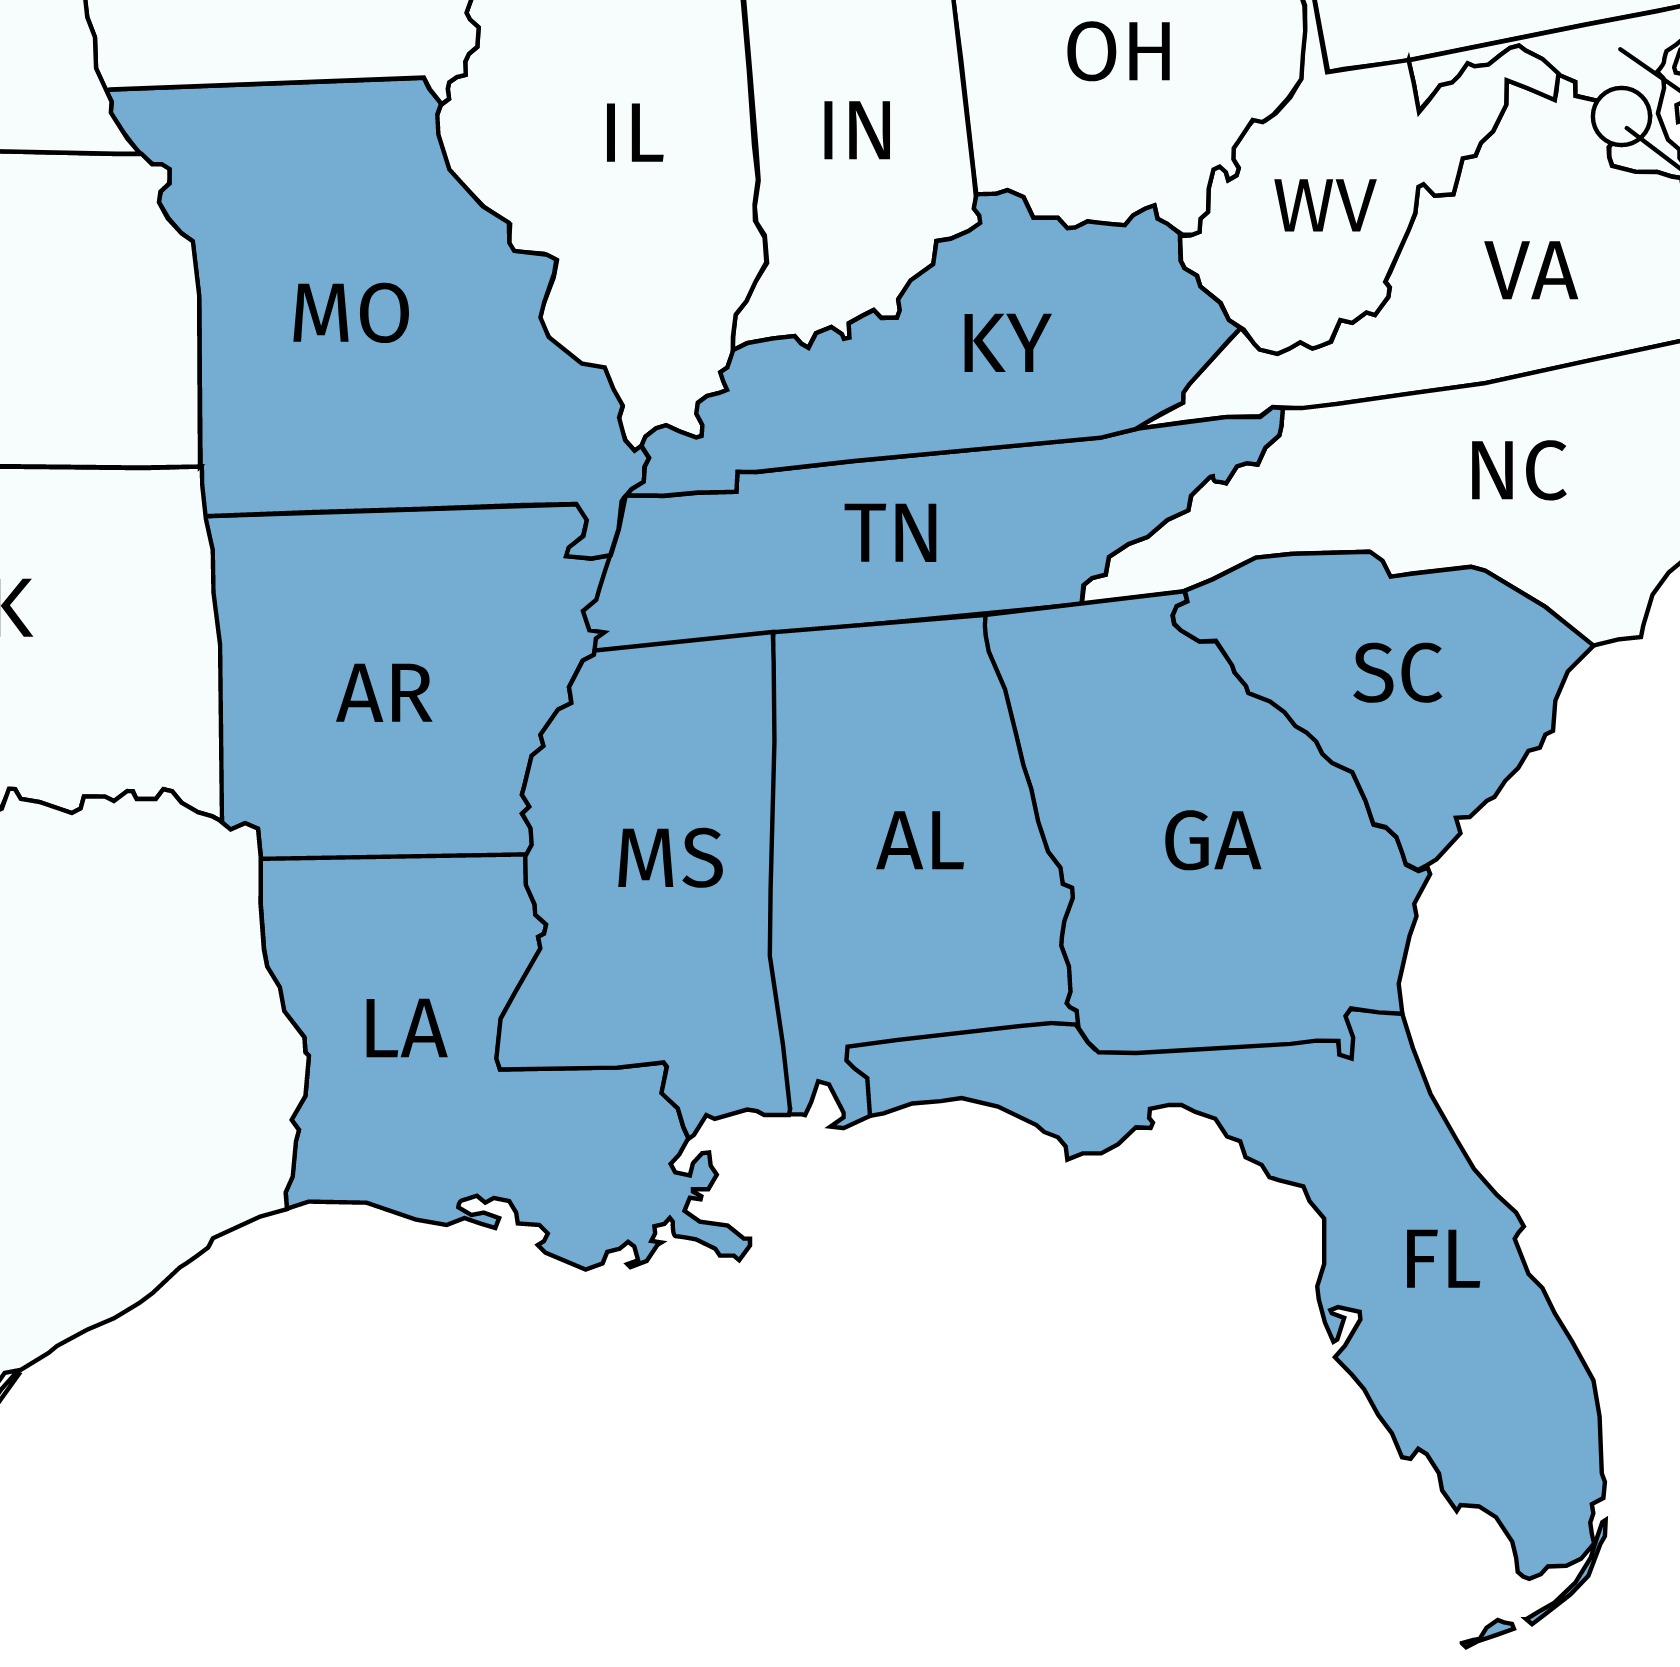
\includegraphics[height=1.7in]{southeast_states2_cropped}
\end{center} \text{} \answer{Yes, starting/ending in MO/SC}

\item France is divided into 18 administrative regions, of which twelve are contiguous.  The map below shows seven of these regions highlighted in blue.  Is there a path that a traveler could take through these regions in such a way that they cross each border between two regions exactly once?
\begin{center}
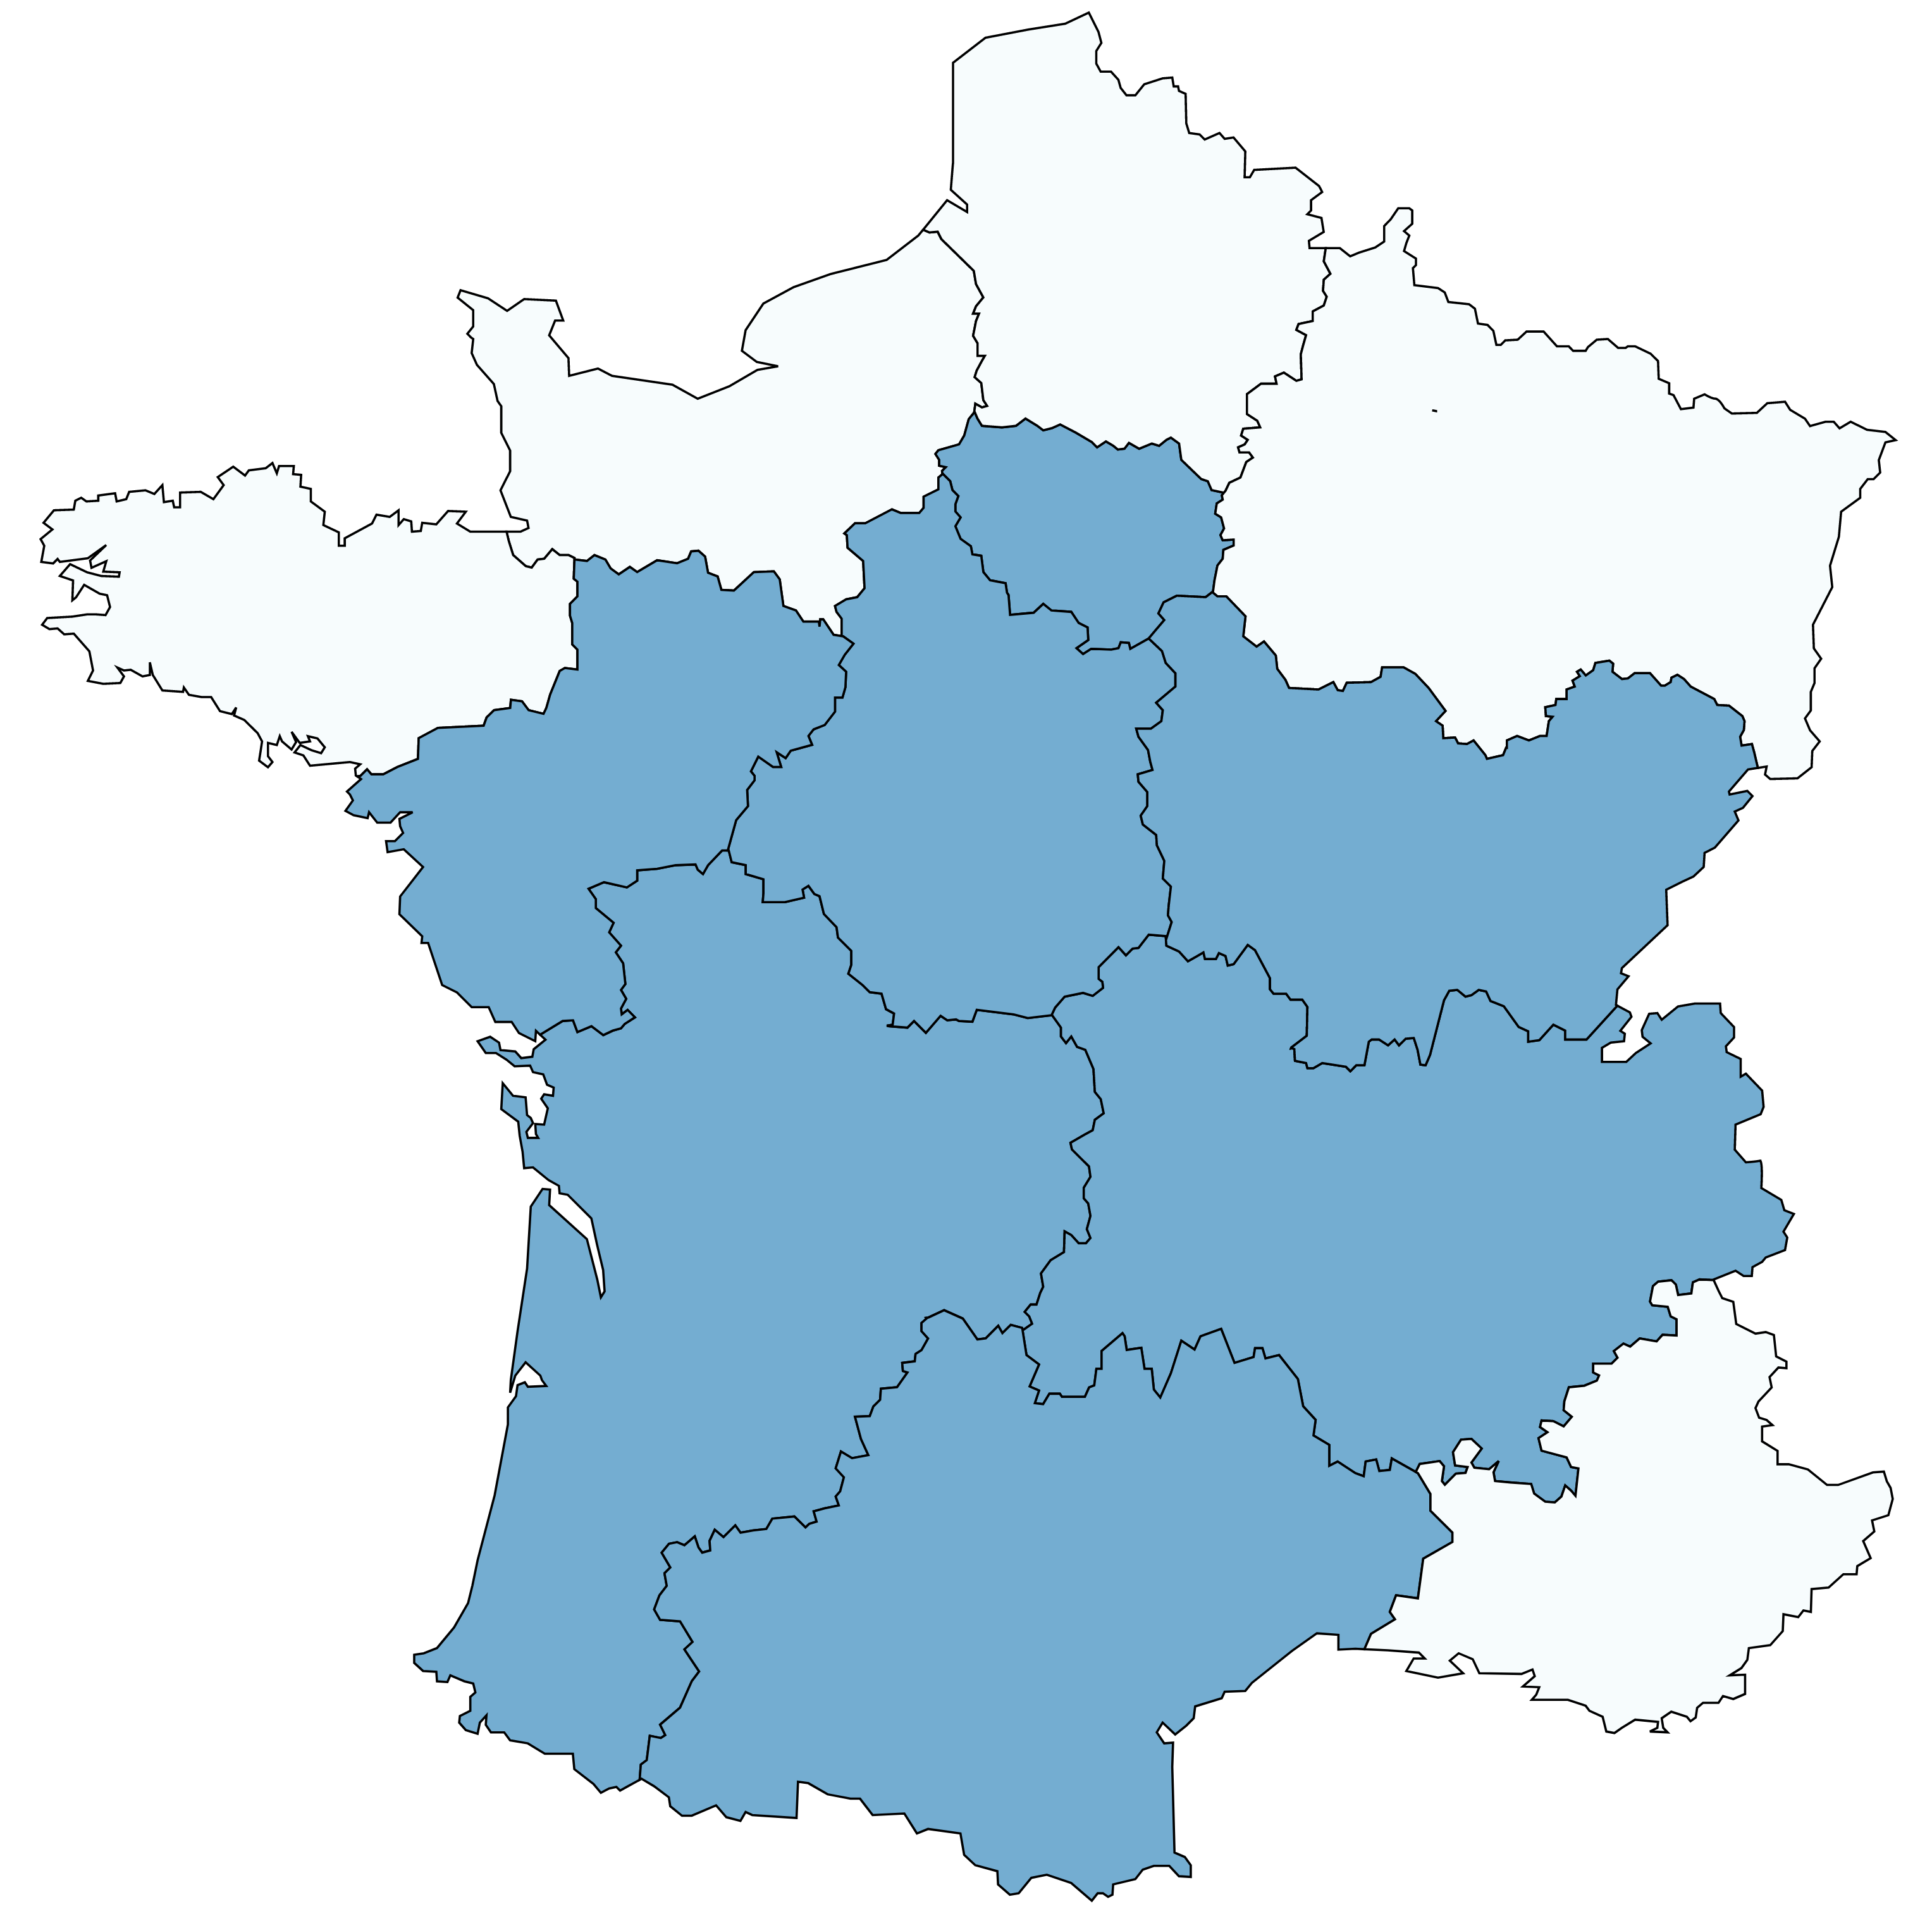
\includegraphics[height=1.6in]{france_states_cropped}
\end{center} \text{} \answer{Yes}
\end{enumerate}

\emph{In problems 22--25, determine whether the given graph has a Hamilton circuit (and draw one if it does).  If not, determine whether it has a Hamilton path (and draw one if so).}
\begin{enumerate}
\setcounter{enumi}{21}

\item \text{} \answer{Hamilton path ($febcad$, for instance)} \begin{center} %22
\begin{tikzpicture}
  \GraphInit[vstyle=simple]
  \tikzset{VertexStyle/.append style={scale=0.3}}
  \SetGraphUnit{1}
  \Vertex{a}
  \SOEA(a){c}
  \NOEA(c){b}
  \SOWE(c){d}
  \SOEA(c){e}
  \EA(e){f}
  
  \extralabel{a}{90}{$a$}
  \extralabel{b}{90}{$b$}
  \extralabel{c}{225}{$c$}
  \extralabel{d}{-90}{$d$}
  \extralabel{e}{-90}{$e$}
  \extralabel{f}{-90}{$f$}
  
  \Edge(a)(b)
  \Edge(a)(c)
  \Edge(a)(d)
  \Edge(b)(c)
  \Edge(b)(e)
  \Edge(c)(e)
  \Edge(d)(e)
  \Edge(e)(f)
\end{tikzpicture}
\end{center}
\pagebreak

\item \text{} \answer{No Hamilton circuit or path} \begin{center} %23
\begin{tikzpicture}
  \GraphInit[vstyle=simple]
  \tikzset{VertexStyle/.append style={scale=0.3}}
  \SetGraphUnit{1.6}
  \Vertex{a}
  \EA(a){b}
  \EA(b){g}
  \SO(a){c}
  \WE(c){e}
  \EA(c){d}
  \EA(d){f}
  
  \extralabel{a}{90}{$a$}
  \extralabel{b}{90}{$b$}
  \extralabel{c}{-90}{$c$}
  \extralabel{d}{-90}{$d$}
  \extralabel{e}{-90}{$e$}
  \extralabel{f}{-90}{$f$}
  \extralabel{g}{90}{$g$}
  
  \Edge(a)(b)
  \Edge(a)(c)
  \Edge(a)(d)
  \Edge(b)(c)
  \Edge(b)(d)
  \Edge(b)(g)
  \Edge(c)(d)
  \Edge(c)(e)
  \Edge(d)(f)
\end{tikzpicture}
\end{center}

\item \text{} \answer{Hamilton circuit ($abcefihgda$, for instance)} \begin{center} %24
\begin{tikzpicture}
  \GraphInit[vstyle=simple]
  \tikzset{VertexStyle/.append style={scale=0.3}}
  \SetGraphUnit{1}
  \Vertex{a}
  \EA(a){b}
  \EA(b){c}
  \SO(a){d}
  \EA(d){e}
  \EA(e){f}
  \SO(d){g}
  \EA(g){h}
  \EA(h){i}
  
  \extralabel{a}{90}{$a$}
  \extralabel{b}{90}{$b$}
  \extralabel{c}{90}{$c$}
  \extralabel{d}{180}{$d$}
  \extralabel[2mm]{e}{15}{$e$}
  \extralabel{f}{0}{$f$}
  \extralabel{g}{-90}{$g$}
  \extralabel{h}{-90}{$h$}
  \extralabel{i}{-90}{$i$}
  
  \Edge(a)(b)
  \Edge(a)(d)
  \Edge(a)(e)
  \Edge(b)(c)
  \Edge(b)(e)
  \Edge(c)(e)
  \Edge(c)(f)
  \Edge(d)(e)
  \Edge(d)(g)
  \Edge(e)(f)
  \Edge(e)(g)
  \Edge(e)(h)
  \Edge(e)(i)
  \Edge(f)(i)
  \Edge(g)(h)
  \Edge(h)(i)
\end{tikzpicture}
\end{center}
\end{enumerate}
